% -*- LaTeX -*-
%
% ----------------------------------------------------------------------
%
% Brad T. Aagaard, U.S. Geological Survey
% Charles A. Williams, GNS Science
% Matthew G. Knepley, University of Chicago
%
% This code was developed as part of the Computational Infrastructure
% for Geodynamics (http://geodynamics.org).
%
% Copyright (c) 2010-2017 University of California, Davis
%
% See COPYING for license information.
%
% ----------------------------------------------------------------------
%

\newcommand{\HRule}{\rule{\textwidth}{0.2em}}
\noindent\MakeUppercase{{\sffamily\Large Computational Infrastructure for Geodynamics (CIG)}}\\
\HRule
\vspace{2em}

\noindent\begin{tikzpicture}
  \node[draw=none,
  inner sep=1.0em,
  fill=mdblue,
  minimum width=0.3333\textwidth,
  scale=3.0,
]{\color{white}\Huge PyLith};
\end{tikzpicture}
{\raggedleft{\Huge User Manual}\\[8pt]
  {\LARGE Version 2.1.4}\\}
{\centering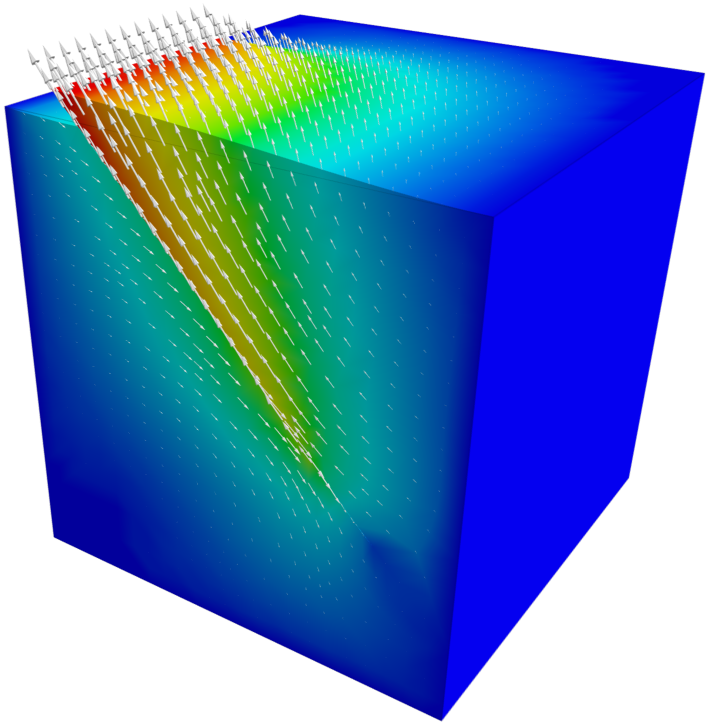
\includegraphics[height=0.5\textheight]{cover/coverimage}\\}
{\raggedleft\LARGE Brad Aagaard \\ Matthew Knepley \\ Charles Williams\\}
\vfill
\noindent{\sffamily\LARGE www.geodynamics.org}\\
\HRule
\thispagestyle{empty}
